\documentclass{article} % For LaTeX2e
\usepackage{nips13submit_e,times}
\usepackage{hyperref}
\usepackage{url}
\usepackage{amsmath}
\usepackage{graphicx}
\usepackage[raggedright]{sidecap}

\title{Learning words through recursive pragmatic reasoning about other agents}

\author{
Nathaniel Smith\thanks{...} \\
School of Informatics\\
University of Edinburgh\\
Edinburgh, Scotland, UK\\
\texttt{nathaniel.smith@ed.ac.uk} \\
\AND
Noah D. Goodman \\
Department of Psychology\\
Stanford University \\
Stanford, CA, USA \\
\texttt{ngoodman@stanford.edu} \\
\And
Michael C. Frank \\
Department of Psychology \\
Stanford University \\
Stanford, CA, USA \\
\texttt{mcfrank@stanford.edu}}

\newcommand{\fix}{\marginpar{FIX}}
\newcommand{\new}{\marginpar{NEW}}

\newcommand{\word}{\text{word}}
\newcommand{\obj}{\text{object}}
\newcommand{\lex}{\text{lexicon}}
\newcommand{\prior}{P_{\text{prior}}(\obj | \text{context})}

% \nipsfinalcopy % Uncomment for camera-ready version

\begin{document}

\maketitle

\begin{abstract}
  Adult language users are remarkably good at making inferences about speakers' intentions in context, and children learning their native language also display substantial pragmatic skill in acquiring the meanings of unknown words. While pragmatic inference and word learning have both been characterized in probabilistic terms, no current models make appropriate inferences about the meanings of words in pragmatically-rich inferential contexts. We describe a model in which language learners assume that they jointly approximate a shared, external lexicon and reason recursively about the goals of others in using this lexicon. This model captures phenomena in word learning and pragmatic inference; it additionally leads to insights about the emergence of communicative systems in conversation and the mechanisms by which pragmatic inferences become incorporated into word meanings.
\end{abstract}

\section{Introduction}

Natural language is a powerful tool for conveying meaning in context. Our utterances are pervasively underspecified. Consider ``it's raining,'' ``I ate some of the cookies,'' or ``can you close the window?'' In each, a listener must go beyond the literal meaning of the words to fill in contextual details (``it's raining here and now''), infer that a stronger alternative is not true (``I ate some but not all of the cookies''), or more generally infer the speaker's communicative goal (``I want you to close the window right now because I'm cold.'').

Following this intuition, theories of pragmatic communication frame the process of language comprehension as inference about the generating goal of an utterance given a rational speaker \cite{grice1975,dale1995,frank2012}. For example, a listener might reason, ``if she had wanted me to think `all' of the cookies, she would have said `all'---but she didn't. Hence `all' must not be true and she must have eaten some {\it but not all} of the cookies.'' This kind of counterfactual reasoning has a recursive character to it: listener models speaker (who may in turn be modeling a listener).

Even before they are proficient language users, children learn the meanings of words from their pattern of use in context. For example, in demonstrations of the ``disambiguation effect,'' a novel word (e.g. ``dax'') is used in a context containing both a novel and a familiar object. From quite young, children tend to make the inference that ``dax'' refers to the novel object \cite{markman1988}. In another demonstration, even young toddlers can extract mappings between words and objects from a pattern of individually-ambiguous co-occurrences between pairs of words and pairs of objects \cite{smith2008}. Taking inspiration from children's learning prowess, recent work in the field of grounded language learning has explored the possibility that even relatively complex word meanings can be inferred from corpus data (e.g. \cite{zettlemoyer2005,chen2008,frank2009,kwiatkowski2010,johnson2012}).

Recursive pragmatic inferences such as those described above could be an important part of language learning.\footnote{Very young children make inferences that are often labeled as ``pragmatic'' in that they involve reasoning about context \cite{clark1988,baldwin1993}, though they also show weaknesses in specific inferences (e.g. strengthening ``some'' to ``some but not all'' \cite{papafragou2003}). Here we remain agnostic about the age at which children are able to make such inferences robustly, as it may vary depending on the linguistic materials being used in the inference \cite{barner2011}.} For example, the disambiguation inference described above can emerge from such reasoning (``why would the speaker have said ``dax'' if there was a word for the known object that she knew I would know'') \cite{clark1988}. In addition, there are a variety of intriguing cases in which listeners seem to create situation- and task-specific ways of referring to particular objects. For example, when asked to refer to idiosyncratic geometric shapes, over the course of an experimental session, participants create conventionalized descriptions that allow them to perform accurately even though they do not begin with a shared label \cite{krauss1964,clark1986}. Yet models of grounded language learning have failed to take pragmatic factors into account.

The goal of our current work is to investigate the possibilities for integrating models of recursive pragmatic reasoning with models of language learning, with the hope of capturing phenomena in both domains. We begin by describing previous models in each domain as well as proposals for bringing the two together. We next simulate findings from the domains of pragmatic inference, word learning, and their intersection (summarized in Table \ref{tab:results}). We end by discussing the implications of our results for work on language change.

\section{Model}

Consider a simple communicative game: two participants each,
separately, view identical arrays of objects. On the
\textit{Speaker's} screen, one object is highlighted; their goal is to
get the \textit{Listener} to click on this item. To do this, they have
available a fixed, finite set of words; they must pick one. The
Listener then receives this word, and attempts to guess which object
the Speaker meant by it.

When modelling human behaviour, it's useful to begin with optimal models; this has the advantage that when we are then forced to deviate from the purely rational approach, it's generally in a theoretically interpretable way. However, multi-agent interactions are notoriously difficult to model in a normative fashion without falling prey to paradox. For example, consider a simple model of the agents in the above game. First we define a \textit{literal listener} agent denoted $L_0$. This agent has a \textit{lexicon} which probabilistically maps words to meanings; specifically, it assigns each word $w$ a vector describing the extent to which this word provides evidence for each object; each entry in the vector is in $(0, 1)$, and together they sum to 1:
\begin{align*}
P_{L_0}(\obj | \word, \lex) &\propto \lex(\word, \obj) \times \prior.
\end{align*}
Confronted with such a listener, a rational (but noisy) speaker should attempt to choose a word which soft-maximizes the probability that the listener will assign to the target object -- possibly modulated by the effort or cost associated with producing this word:
\begin{align*}
P_{S_1}(\word | \obj, \lex) &\propto \exp\Big(\lambda \big(\log P_{L_0}(\obj | \word, \lex) - \text{cost}(\word)\big)\Big).
\end{align*}
But if this is how the speaker will behave, then it's not rational for a listener to implement the $L_0$ strategy. Instead, to best determine what object was intended, they should use Bayes rule to invert the speaker's decision procedure:
\begin{align*}
P_{L_2}(\obj | \word, \lex) &\propto P_{S_1}(\word | \obj, \lex) \times \prior.
\end{align*}
Now the paradox becomes apparent. Given such a listener, it's no longer rational for the speaker to implement strategy $S_1$; instead, they should implement strategy $S_3$ which replaces the $P_{L_0}$ term with $P_{L_2}$. And then the listener ought to implement $L_4$, and so on.

One computationally expensive option is to continue iterating such strategies until one reaches a fixed point equilibrium. But, while this guarantees each agent will behave normatively given the other agent's strategy, there is no guarantee that such a strategy will be optimal for the system as a whole; equilibria strategies make up only a small subspace of all possible strategies. Nor is there much evidence the humans find such equilibria; their behaviour in language games (and in other games XX p-beauty) can be well-modeled as implementing $S_n$ or $L_n$ for some small $n$ \cite{frank2012}. Here we adopt $n = 3$ for speakers and $n = 2$ for listeners.

Given such a model, it's conceptually straightforward for a listener to learn to understand a speaker -- the listener simply puts a prior on the speaker's lexicon, and updates it based on the speaker's utterances and whatever information the listener can glean about their intended meaning.

\begin{align*}
  P_L(\obj | \word) &= P_{S_{n-1}}(\word | \obj, \text{L's data}) \times \prior \\
    &= \sum_\lex P_{S_{n-1}}(\word | \obj, \lex) \times P(\lex | \text{L's data}) \times \prior \\
    &= P_{L_n}(\obj | \word, \text{L's data}). \\
  P_S(\word | \obj) &\propto \exp\Big(\lambda \big(\log P_{L_n}(\obj | \word, \text{S's data}) - \text{cost}(\word)\big)\Big).
\end{align*}

-- if they have the same data, $S$ is rational and $L$ is as close to rational as is possible given a finite recursion depth, i.e., if $S$ recursed one fewer times then $L$ would be rational. In particular, this describes all of the one-shot language games that have been considered in the literature to date, where neither agent has the time to acquire any data.
-- if one actually does know the lexicon and the other is relatively ignorant, as in the child language learning case, then both are rational (with the same caveat).
-- but in general, in multi-turn interactions, their beliefs will display some complicated

% This suggest a simple probabilistic model. Given any particular
% decision procedure used by the Speaker $S$, the optimal way for the
% Listener $L$ to judge the probability of each object is to invert this
% decision procedure using Bayes' rule, taking into account the prior
% likelihood of each object:
% \begin{align*}
% P_L(\obj | \word) &\propto P_S(\word | \obj) P_{\text{prior}}(\obj |
% \text{context})
% \end{align*}
% $S$, meanwhile, being herself a rational Bayesian agent, chooses her
% word so as to soft-maximize a utility function $U(\word | \obj)$. She
% gains utility if $L$ is likely to understand her; she loses utility if
% the word is particularly costly to say (e.g., it may be long).
% \begin{align*}
% P_S(\word | \obj) &\propto \exp \lambda U(\word | \obj) \\
% U(\word | \obj) &= \log P_L(\obj | \word) - \text{cost}(\word)
% \end{align*}
% The degree to which she optimizes this utility is controlled by the
% softmax parameter $\lambda$. If $\lambda = 1$ and all words cost the
% same, then her probability of producing a word will be proportional to
% the likelihood that it will cause $L$ to reach the correct
% interpretation; as $\lambda$ increases, she becomes more likely to
% choose the word which maximizes this likelihood. (We somewhat
% arbitrarily set $\lambda = 3$ throughout.)

% This model as stated satisfies various normative criteria for each
% agent individually, but suffers from a serious flaw that is intrinsic
% to such multi-agent situations: $S$'s decision procedure depends on
% $L$'s interpretive procedure, and vice-versa. If $S$ and $L$ want to
% both be optimal simultaneously, then they must restrict themselves to
% a low-dimensional subset of all available strategies. They must each choose
% a strategy with the property that optimal counterpart of its optimal
% counterpart is the original strategy. Finding such an equilibrium is
% computationally non-trivial, and, even if found, there is no guarantee
% that it will be optimal in any global sense. \cite{frank2012}
% therefore propose an approximation to this model, in which $L$ and $S$
% each perform a finite number of recursions, with $S_i$ reasoning about
% $L_{i-1}$, who reasons about $S_{i-2}$ and so forth, until reaching
% $L_0$, who interprets words according to an arbitrary rule (their
% \textit{literal meaning}). In our case, we instantiate this as a
% matrix (the \textit{lexicon}) with one column per object, and in which
% each row represents the meaning of a particular word as a set of
% values in $(0, 1)$ such that $\sum_\obj \lex(\word, \obj) = 1$.\footnote{In this model, words refer directly to objects; more realistically, words should refer to some sort of abstract semantic features, which in turn refer to objects. However, this simplification is without loss of generalization; we can interpret this model as marginalizing over such a representation, with our literal $P(\obj | \word) = \sum_\text{features} P(\obj | \text{features}) P(\text{features} | \word)$.}  Formally, we have:
% \begin{align*}
% P_{L_0}(\obj | \word) &= \lex(\word, \obj) P_{\text{prior}}(\obj | \text{context}). \\
% P_{S_i}(\word | \obj) &\propto \exp\Big(\lambda \big(\log P_{L_{i - 1}}(\obj | \word) - \text{cost}(\word)\big)\Big) \\
% P_{L_i}(\obj | \word) &\propto P_{S_{i-1}}(\word | \obj) P_{\text{prior}}(\obj | \text{context})
% \end{align*}
% This approach neatly avoids the infinite regress, and does well at predicting human behaviour in language games \cite{frank2012} and other multi-agent games (XX p-beauty). The minimal degree of recursion required to produce the effects we consider here is $S_3$ and $L_2$, and this what we use in the following.

% When we consider adding learning to this model, however, we encounter a new and related problem. It's straightforward in principle to put a prior on $\lex(\word, \obj)$, and allow an agent to learn the 

At each stage, $S_i$ defines a causal model for utterances described
by a simple Bayes net, and $L_{i+1}$ does Bayesian inference over this net. But the likelihood function in $S_i$'s model is very complicated, and includes equations derived from considering how a hypothetical $L_{i-1}$ would interpret utterances if they were doing rational inference about another hypothetical causal agent $S_{i-2}$.

extensional as marginalization over intensional


we use $S_3$, $L_2$ and $\lambda = 3$.

\subsection{Naive literal learner model}



To see how
Make $L_0$ uncertain about values in $\lex(\word, \obj)$, impose a prior, and then

Needs feedback

can't switch roles from speaker to listener

knocks out the lexical uncertainty/horn implicature results (because you can only have uncertainty at one level)

something wrong about taking evidence from the pragmatic speaker and using it to train the literal listener

\subsection{``Social anxiety'' model}

\section{Experiments: Pragmatic and word learning phenomena}

In this section, we describe the coverage of our pragmatic learning model on phenomena previously investigated with the pragmatics and word learning components of the model. To summarize these simulations: the pragmatic learning model reproduces previous findings and provides some new insights into the ``disambiguation'' phenomenon described above. 

\begin{table}[t]
\label{tab:results}
\begin{center}
\begin{tabular}{lccccc}
\hline \\
Phenomenon & Ref. & WL & PI & Lifted PI  & PIL \\
\hline
Specificity implicature & \cite{grice1975} &  & x &x & x\\
Horn implicature & \cite{horn1984} & &  & x& x\\
Cross-situational learning & \cite{smith2008} & x& & & x \\
Disambiguation effect & \cite{markman1988} &x  & & & x \\
Disambiguation without mapping & \cite{horst2008} &  & & & x \\
Emergence of communicative equilibria & \cite{galantucci2005} & & & & x \\
Lexicalization of Horn implicature & \cite{horn1984} & & & & x \\
Lexicalization of specificity implicature & \cite{levinson2000} & & & & x \\
\hline
\end{tabular}
\end{center}
\caption{Empirical results and references. WL refers to the word learning model of \cite{frank2009}; PI refers to the pragmatic inference model of \cite{frank2012}; Lifted PI refers to the pragmatic inference model of \cite{bergen2012}, and PIL refers to the pragmatic inference and learning model described here.  }

\end{table}

\subsection{Specificity implicature}

Many sets of words in natural language form scales in which each term refers to successively stronger restrictions on the situations compatible with the term. ``Some'' and ``all'' form a scale of this type. While ``I ate some of the cookies'' is compatible with the followup ``in fact, I ate {\it all} of the cookies,'' the reverse is not true. ``Might'' and ``must'' are another example, as are ``OK,'' ``good,'' and ``excellent.'' All of these scales allow for {\it scalar implicatures} \cite{grice1975}: if a speaker uses a weaker term, a listener is licensed to infer that the stronger term was not true in this situation. So although ``I ate some of the cookies'' could in principle be compatible with eating all of them, the listener is lead to believe that ``some but not all'' is the likely state of affairs. We use the term {\it specificity implicature} here (following \cite{bergen2012}) to denote that we are agnostic about whether such implicatures are conventionalized or whether they use a contextually-defined scale.

The recursive pragmatic reasoning portions of our model capture findings on specificity implicature. Consider a representation of scalar implicature as a matrix 
$\left[
    \begin{array}{cc}
      1 & 1 \\
      0 & 1
    \end{array} 
  \right]$,
where rows show the terms ``some'' and ``all'' and columns indicate worlds where {\sc some} and {\sc all} are true, respectively, capturing the regularity that ``some'' can be said of situations where {\sc all} is actually the case. Assuming uniform costs for the two words and uniform priors, each recursion of listener modeling speaker reduces the probability that ``some'' will be used to refer to {\sc all}. Using the fixed parameters employed in our other simulations results in speaker use probabilities of 
$\left[
    \begin{array}{cc}
      1.00 & 0.00 \\
      0.00 & 1.00
    \end{array} 
  \right]$
and listener interpretation probabilities of 
$\left[
    \begin{array}{cc}
      .86 & .14 \\
      .03 & .97
    \end{array} 
  \right]$.

% Simulation parameters:
%   prior on meaning of "some": dirichlet(10, 10)
%   prior on meaning of "all": dirichlet(1, 10)
%
% How speaker refers to "some" and "all" objects:
% array([[  9.99951162e-01,   2.87541198e-03],
%        [  4.88378335e-05,   9.97124588e-01]])
%
% How listener interprets "some" and "all" words:
% array([[ 0.86214895,  0.13785105],
%        [ 0.03151434,  0.96848566]])

\subsection{Horn implicature}

XX note the relation to BGL model; they need uncertainty in the middle of the pragmatics specifically, which is where we end up putting it for other reasons. And in Bayesian framework uncertainty and learning must always coincide. Also the intuition that this is a general property of uncertainty for soft-max agents -- if you don't know where you are, good worlds have more peaked utility distributions than bad worlds, and thus more consistent behaviour by other agents, so on average when you're guessing what other agents will do, good worlds contribute more to your average than bad worlds.

Horn implicatures are inferences where the critical factor is not the extension of the words in context (as in scalar implicatures), but instead the relative cost of two expressions. In Horn's example, ``Lee got the car to stop'' implies that Lee used an unusual method (e.g. not the brakes) because, had he used the brakes, the speaker would have chosen the simpler and shorter (less costly) expression, ``Lee stopped the car.'' In other words, the costly expression is assumed to be associated with the unusual outcome.

Such an implicature again arises naturally from our model. We create a situation in which expressions have differential costs (e.g. $[.5~1.0]$) and referents have differential probabilities (e.g. $[.8~.2]$). At the settings used throughout the manuscript, speakers in such a situation choose simple words to refer to common referents at different rates than for uncommon references. This situation breaks the symmetry though does not result in as dramatic a diagonal as in the specificity implicature, e.g. for the speaker, \footnote{Rows indicate words and columns indicate referents. For speakers, columns are normalized to indicate a distribution over words to be produced given referents, and for listeners rows are normalized to indicate a distribution on referents given words heard.}
$\left[
    \begin{array}{cc}
      .88 & .54 \\
      .12 & .46
    \end{array} 
  \right]$ 
and for the listener,
$\left[
    \begin{array}{cc}
      .77 & .23 \\
      .65 & .35
    \end{array} 
  \right]$. See Section \ref{sec:hornlearn} for the consequences of repeating this implicature until it is lexicalized.


% Simulation parameters:
%   word costs: 0.5, 1.0
%   object prior: 0.8, 0.2
%
% How speaker refers to "common" and "rare" objects:
% array([[ 0.88491473,  0.53858973],
%        [ 0.11508527,  0.46141027]])
%
% How listener interprets "cheap" and "expensive" words:
% array([[ 0.77458316,  0.22541684],
%        [ 0.64702551,  0.35297449]])

\subsection{Statistical cross-situational word learning}

Even very young children can learn words from individually ambiguous situations, e.g. where multiple words are spoken and multiple objects are present \cite{smith2008}. While no individual situation gives away the mapping, the pattern of co-occurrences between words and objects allows for learning. Our current model reproduces this pattern of results, converging to correct lexical mappings from ambiguous evidence. A representative simulation is shown in Fig. \ref{fig:cross-sit}.

\begin{SCfigure}[2.5]
  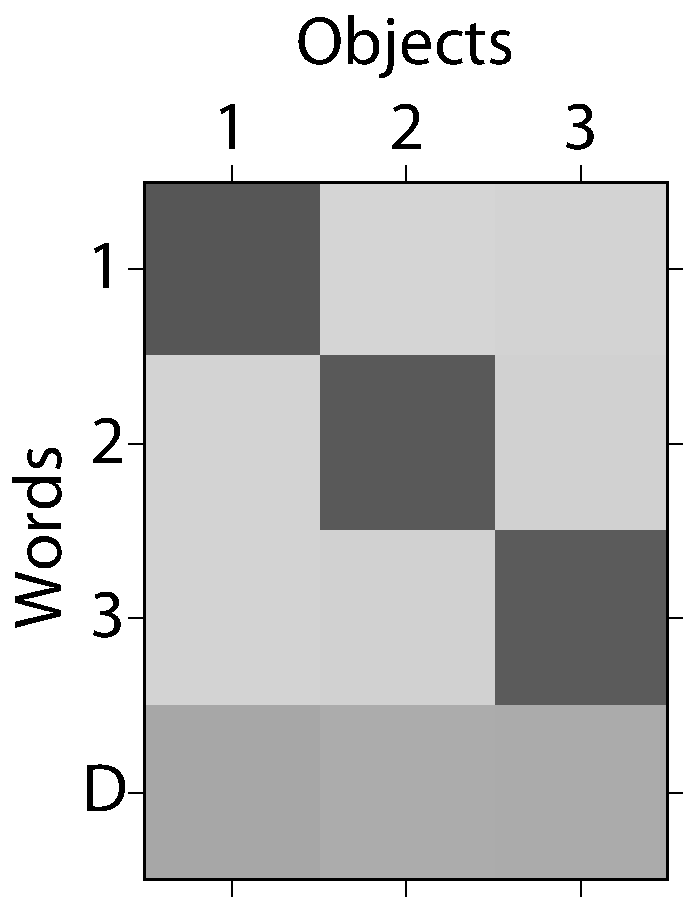
\includegraphics[width=0.2\textwidth]{figures/cross-sit-mod.pdf}
  \caption{Results from a simulation of cross-situational word learning. The posterior distribution over the learner's lexicon (diagonal entries are correct for word/object pairs 1 -- 3; word D is a distractor). Training data were situations including two of the three objects and a single word, either the distractor or a word matching one of the two objects.}
  \label{fig:cross-sit}
\end{SCfigure}

\subsection{Disambiguation using known words}

\begin{SCfigure}[1]
  \centering
  % 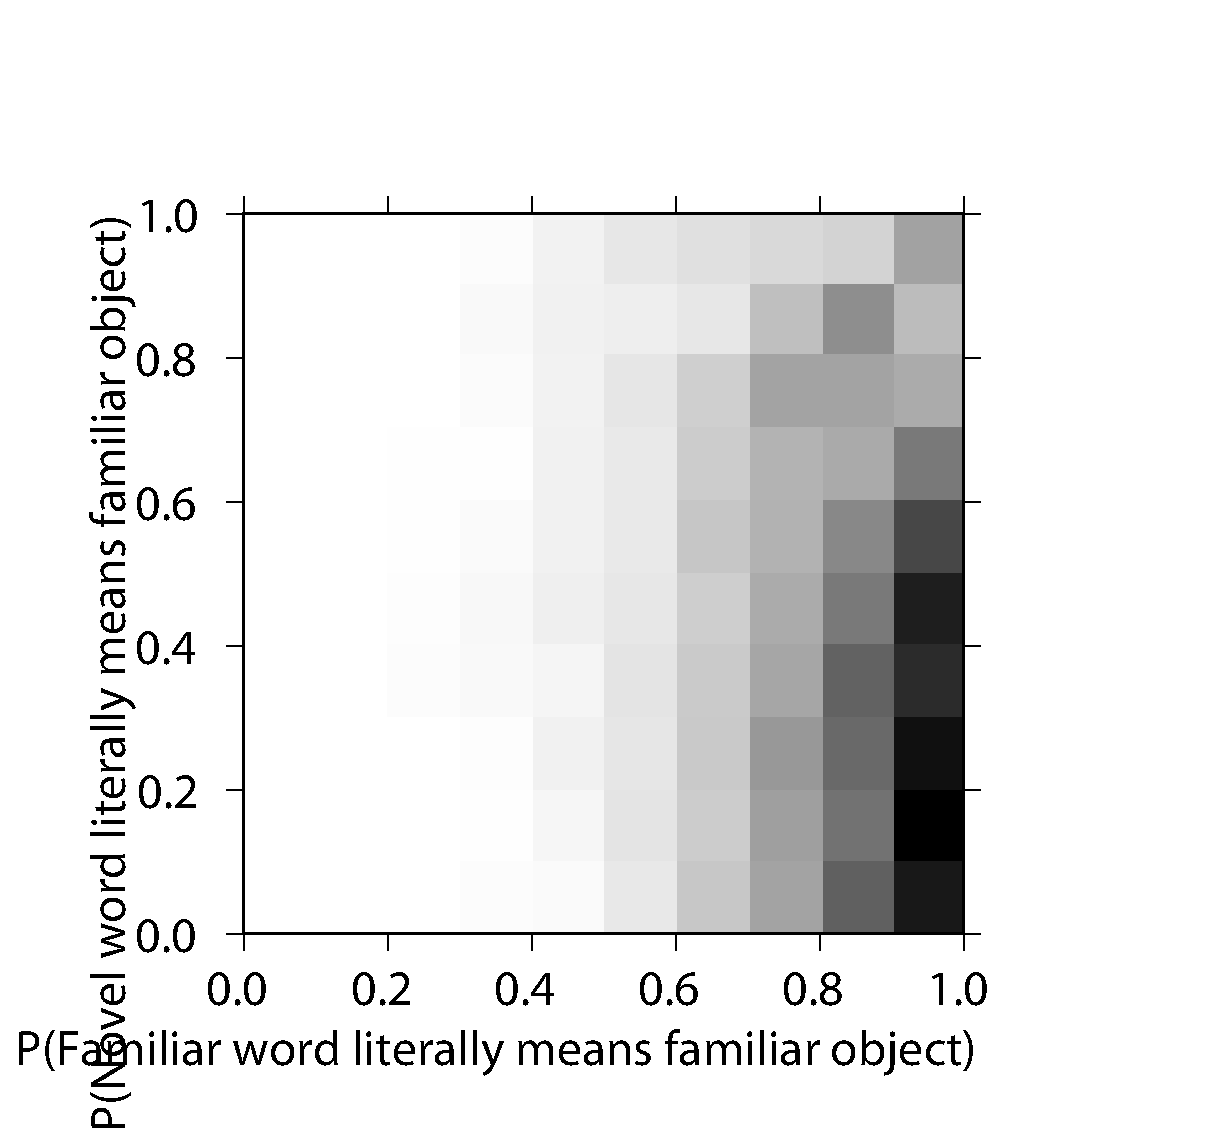
\includegraphics[width=0.24\textwidth]{figures/ME-1dax.pdf}
  % 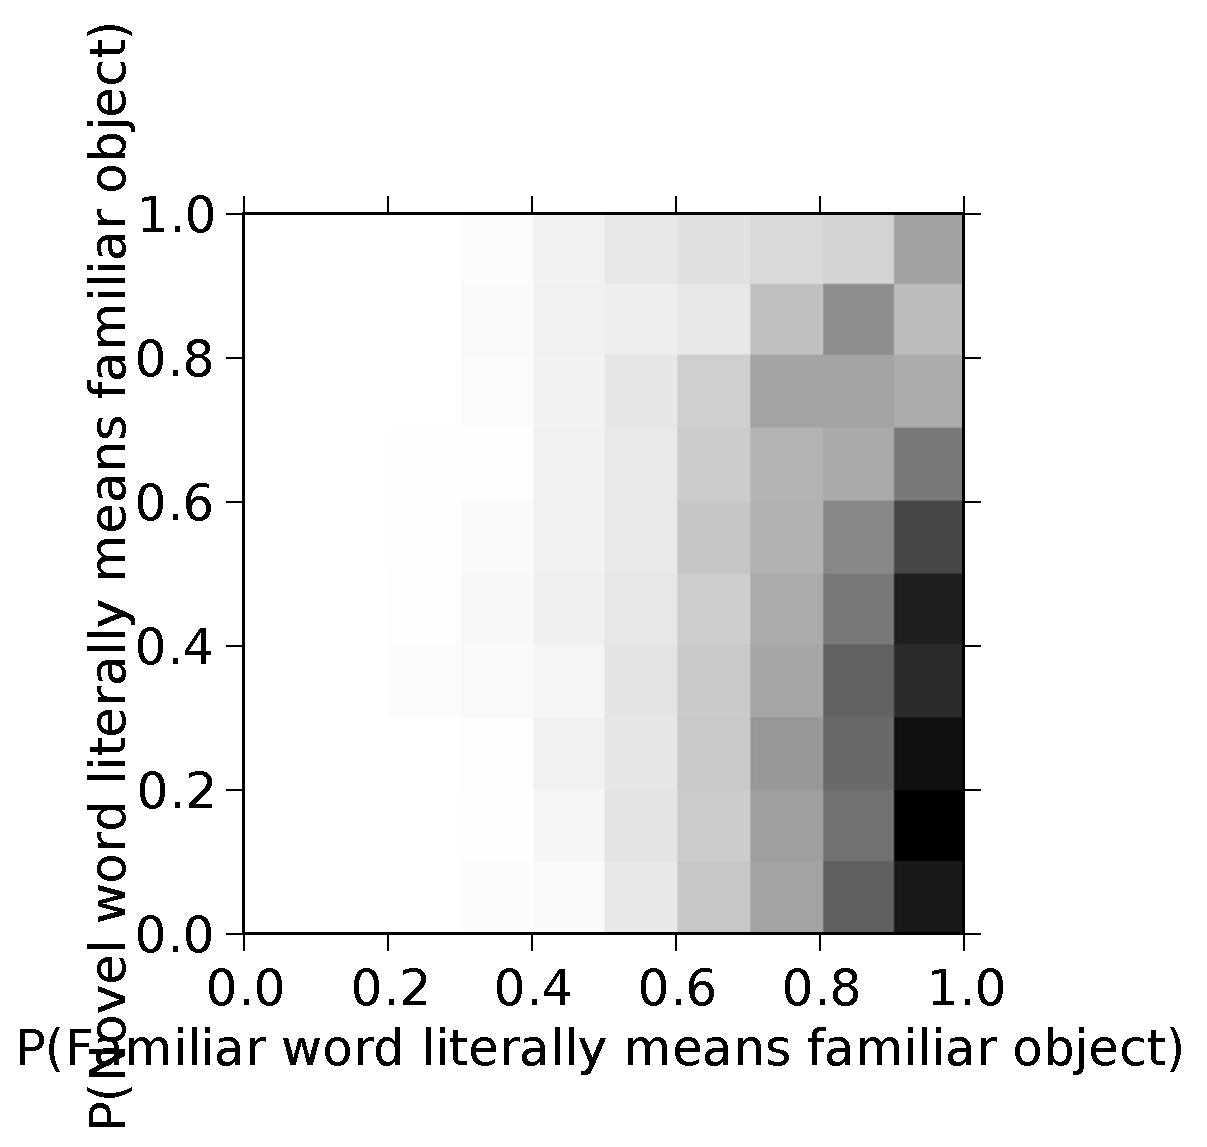
\includegraphics[width=0.24\textwidth]{figures/ME-flat-10dog-10dax.pdf}
  % 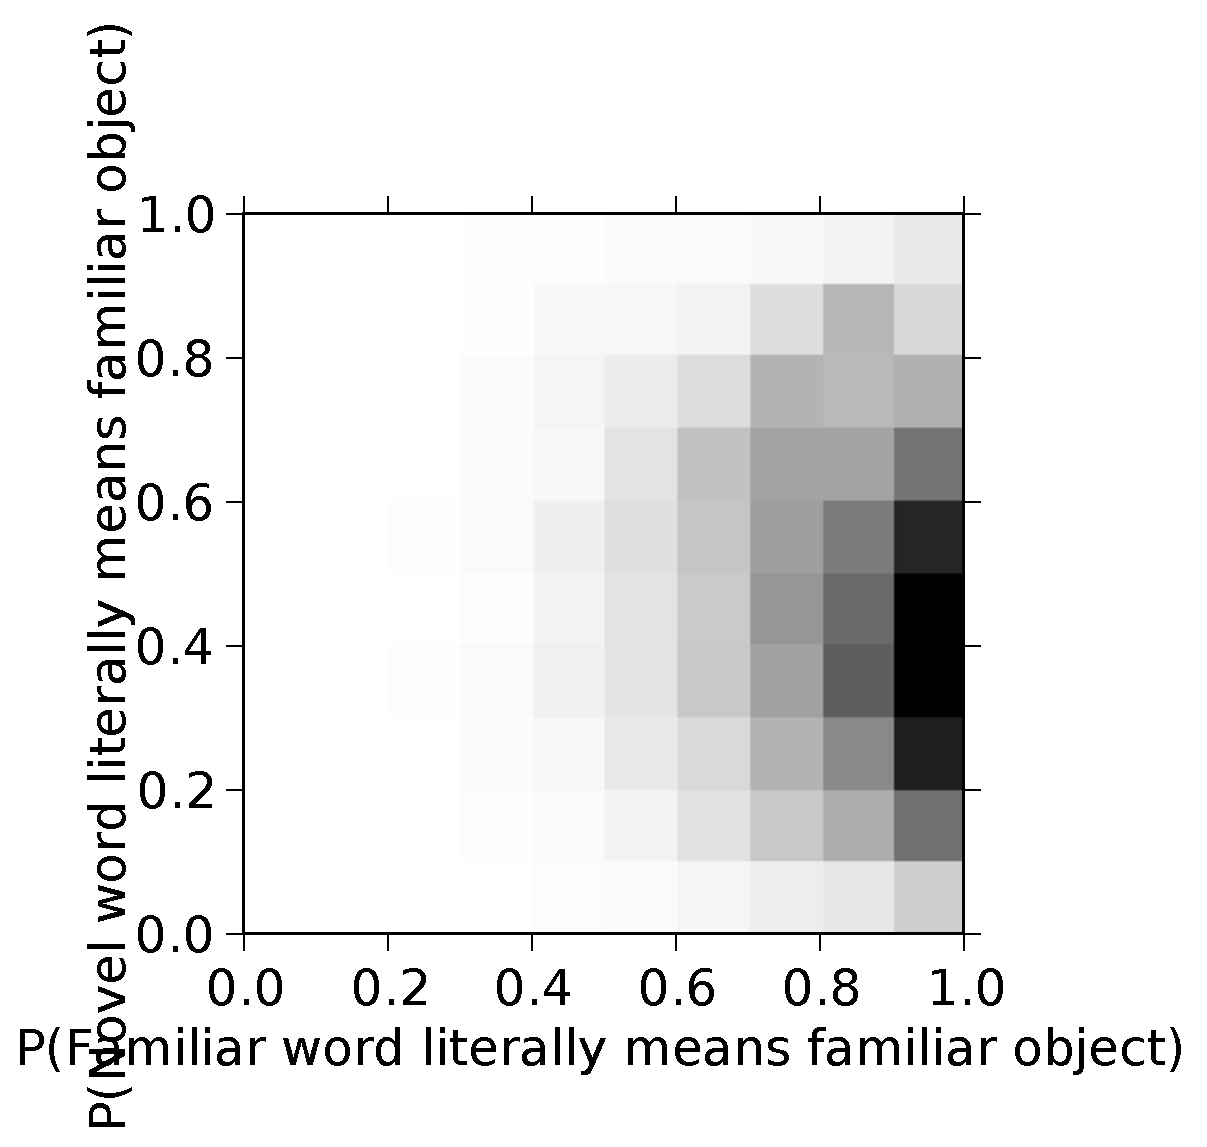
\includegraphics[width=0.24\textwidth]{figures/ME-antisparse-10dog-10dax.pdf}
  % 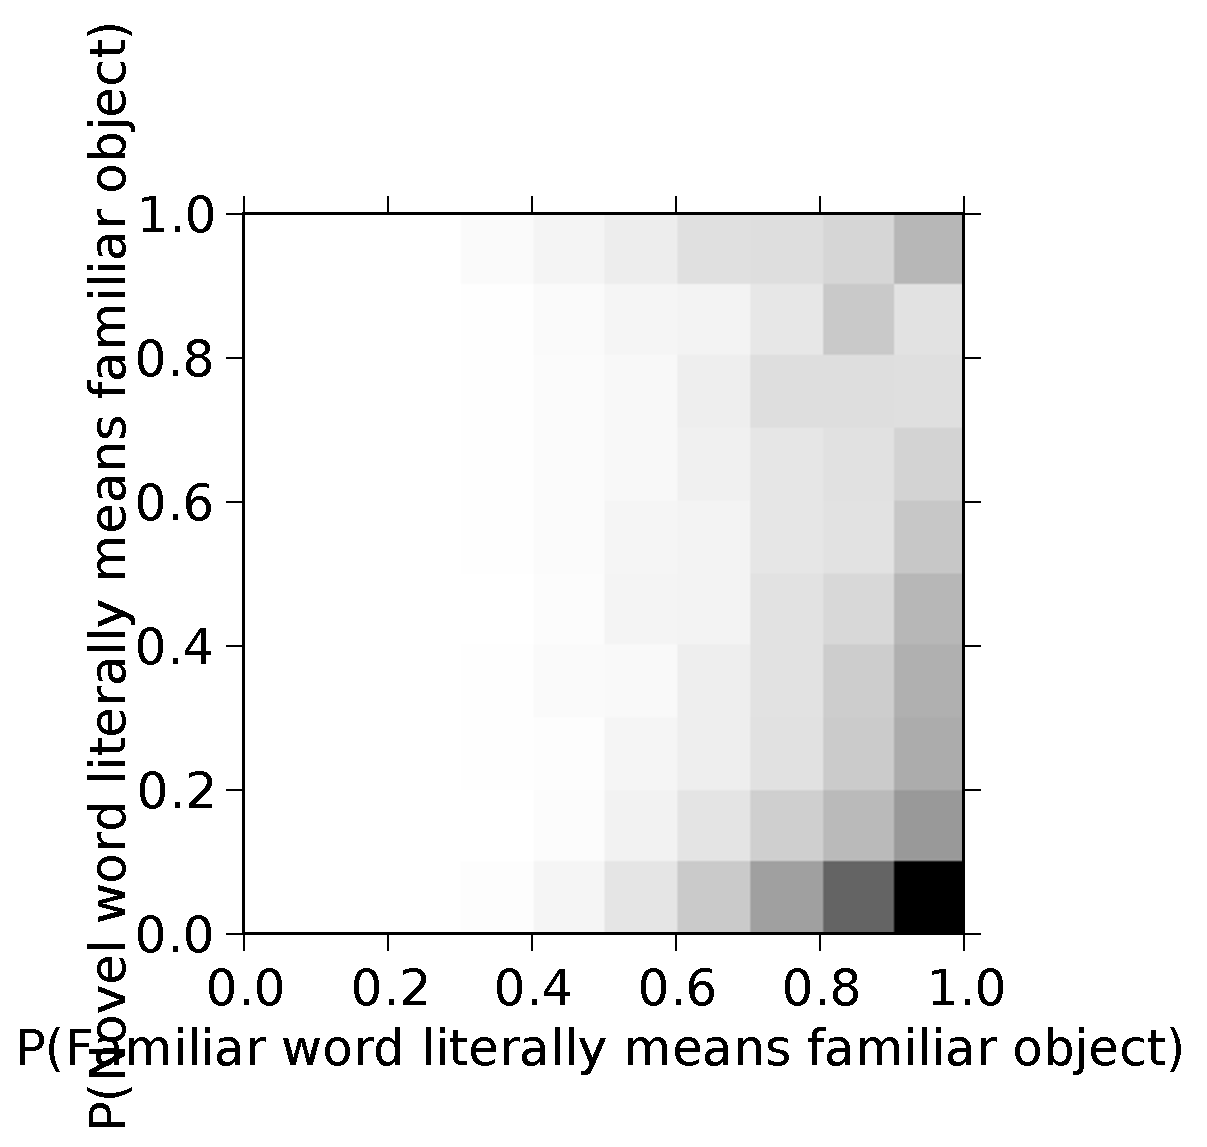
\includegraphics[width=0.24\textwidth]{figures/ME-sparse-10dog-10dax.pdf}
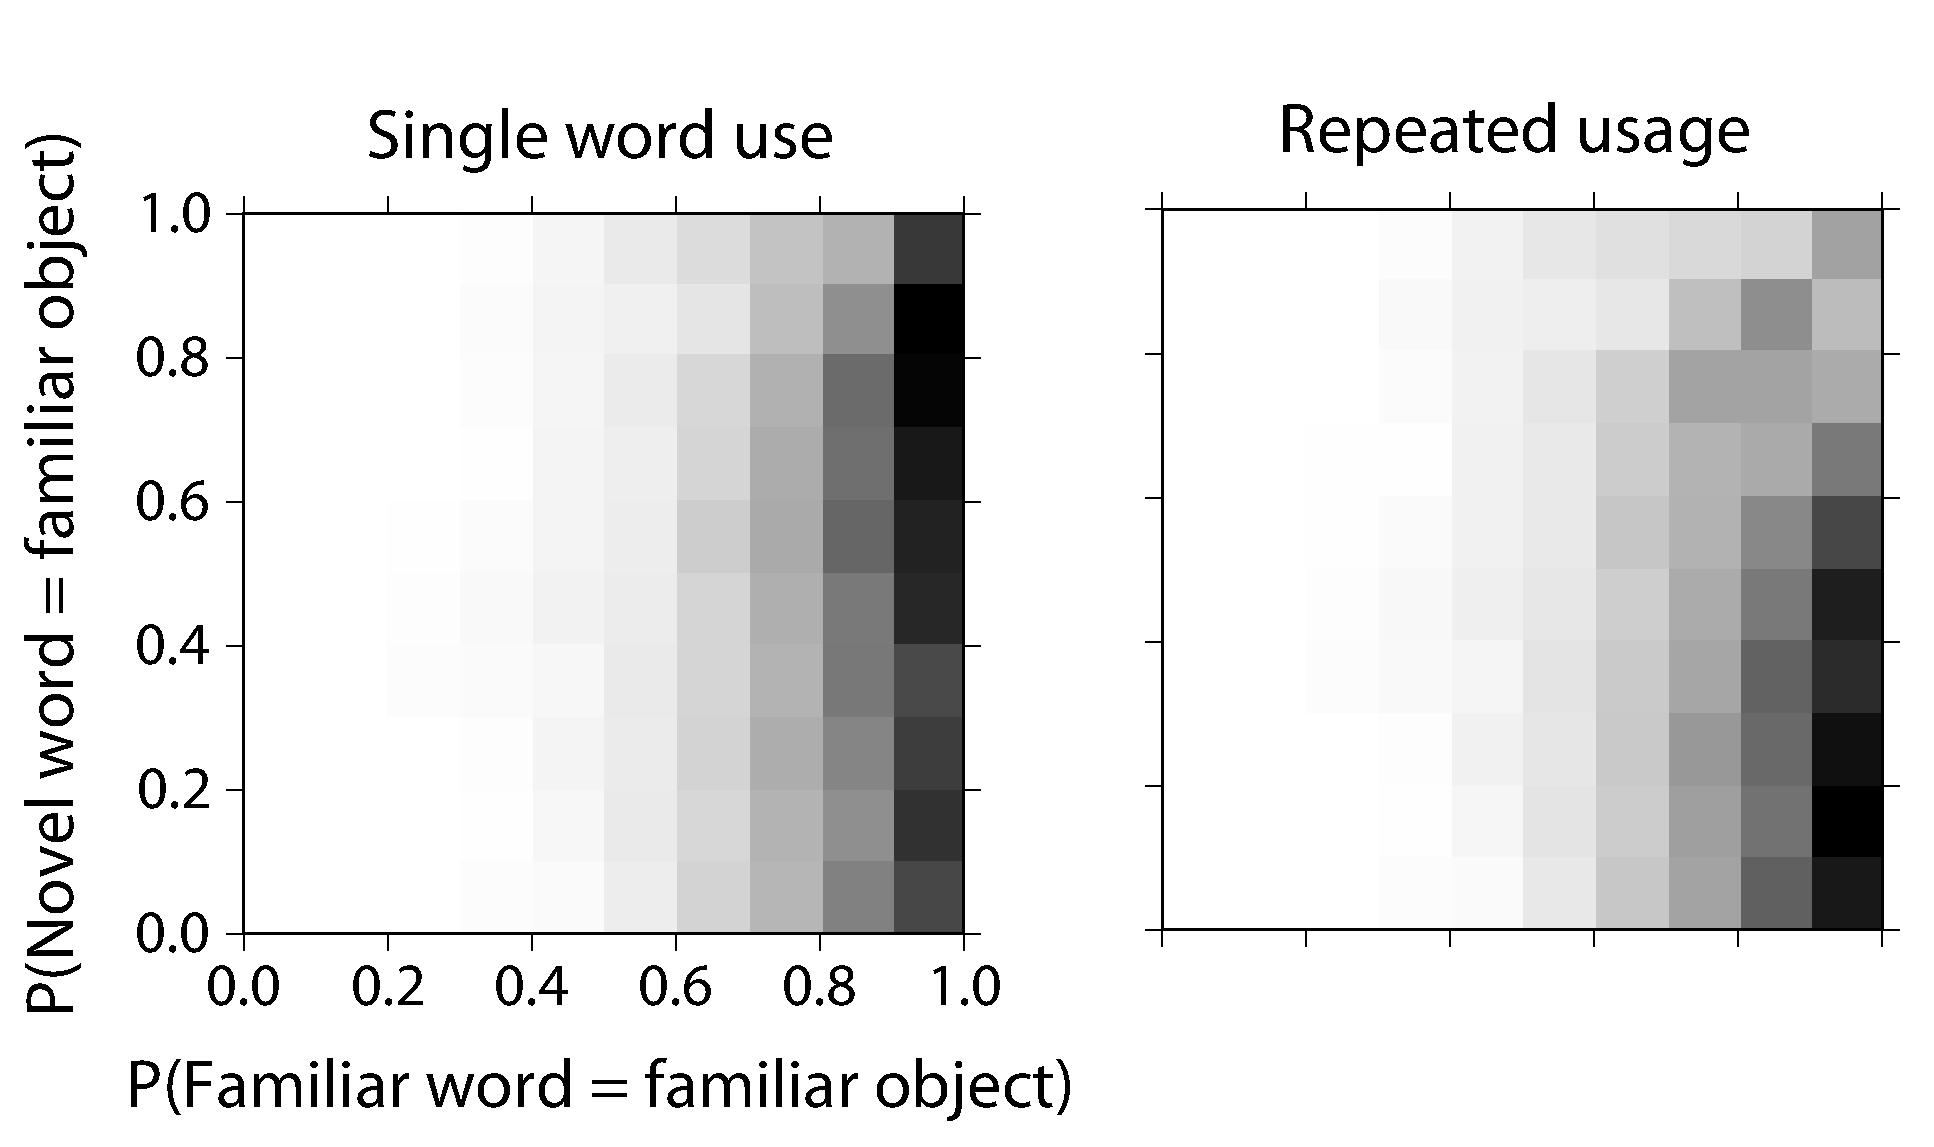
\includegraphics[width=.6\textwidth]{figures/ME-composite-small.pdf}
  \caption{Results for simulations of the ``disambiguation'' phenomenon. A novel word is used in a situation with a novel object and a familiar object. Each plot shows the joint posterior probability that the familiar word refers to the familiar object (horizontal) and that the novel word refers to the familiar object (vertical). Left plot shows the posterior after a single situation; right plot shows multiple situations. 
%The right middle plot shows the posterior after a single situation given either a prior that makes it likely that there are words referring to both the novel and familiar objects (perhaps because the two objects are physically similar; the right plot shows a situation where the prior makes it unlikely that a word refers to both (objects dissimilar). 
}
  \label{fig:me}
\end{SCfigure}

Children, when presented with both a novel and a familiar object (e.g. an eggbeater and a ball), will treat a novel label (e.g. ``dax'') as referring to the novel object, for example by supplying the eggbeater when asked to ``give me the dax'' \cite{markman1988}. This phenomenon is sometimes referred to as ``mutual exclusivity'' or even ``Fast mapping,'' and many distinct theoretical accounts have been proposed in the psychological literature. Simple probabilistic word learning models can produce a similar pattern of findings \cite{frank2009}, often due to the kinds of ``explaining away'' type phenomena that are observed in such models. But all such models assume that learners in fact retain the mapping between word and object that is demonstrated in the experimental situation; this observation is contradicted, however, by evidence that children often do not retain the mappings that are demonstrated by their inferences in the moment \cite{horst2008}. 

Our model provides an intriguing possible explanation of this finding: given a single disambiguation situation, the model gives a substantial probability (e.g. 75\%) that the speaker is referring to the novel object. Nevertheless, integrating across lexicons reveals that this probability is not due to learning that the novel word refers to this object (as shown in Fig. \ref{fig:me}, left): instead, it comes in part from a specificity implicature because the listener knows that the familiar word \emph{does not} refer to the novel object--hence the novel word (even if it refers to the familiar object as well) is the best way to refer to the novel object. Nevertheless, on repeated exposure to the same novel word, novel object situation, the model does lexicalize this inference (Fig. \ref{fig:me}, right). 

% Novel word means: Familiar object: 25.5%. Novel object: 74.5%.
% To anti-sparse listener, novel word means: Familiar object: 21.4%. Novel object: 78.6%.
% To sparse listener, novel word means: Familiar object: 30.5%. Novel object: 69.5%.

\section{Experiments 2: Lexical learning in pragmatic contexts}

\subsection{Emergence of communicative equilibria}

\begin{figure}[t]
\centering
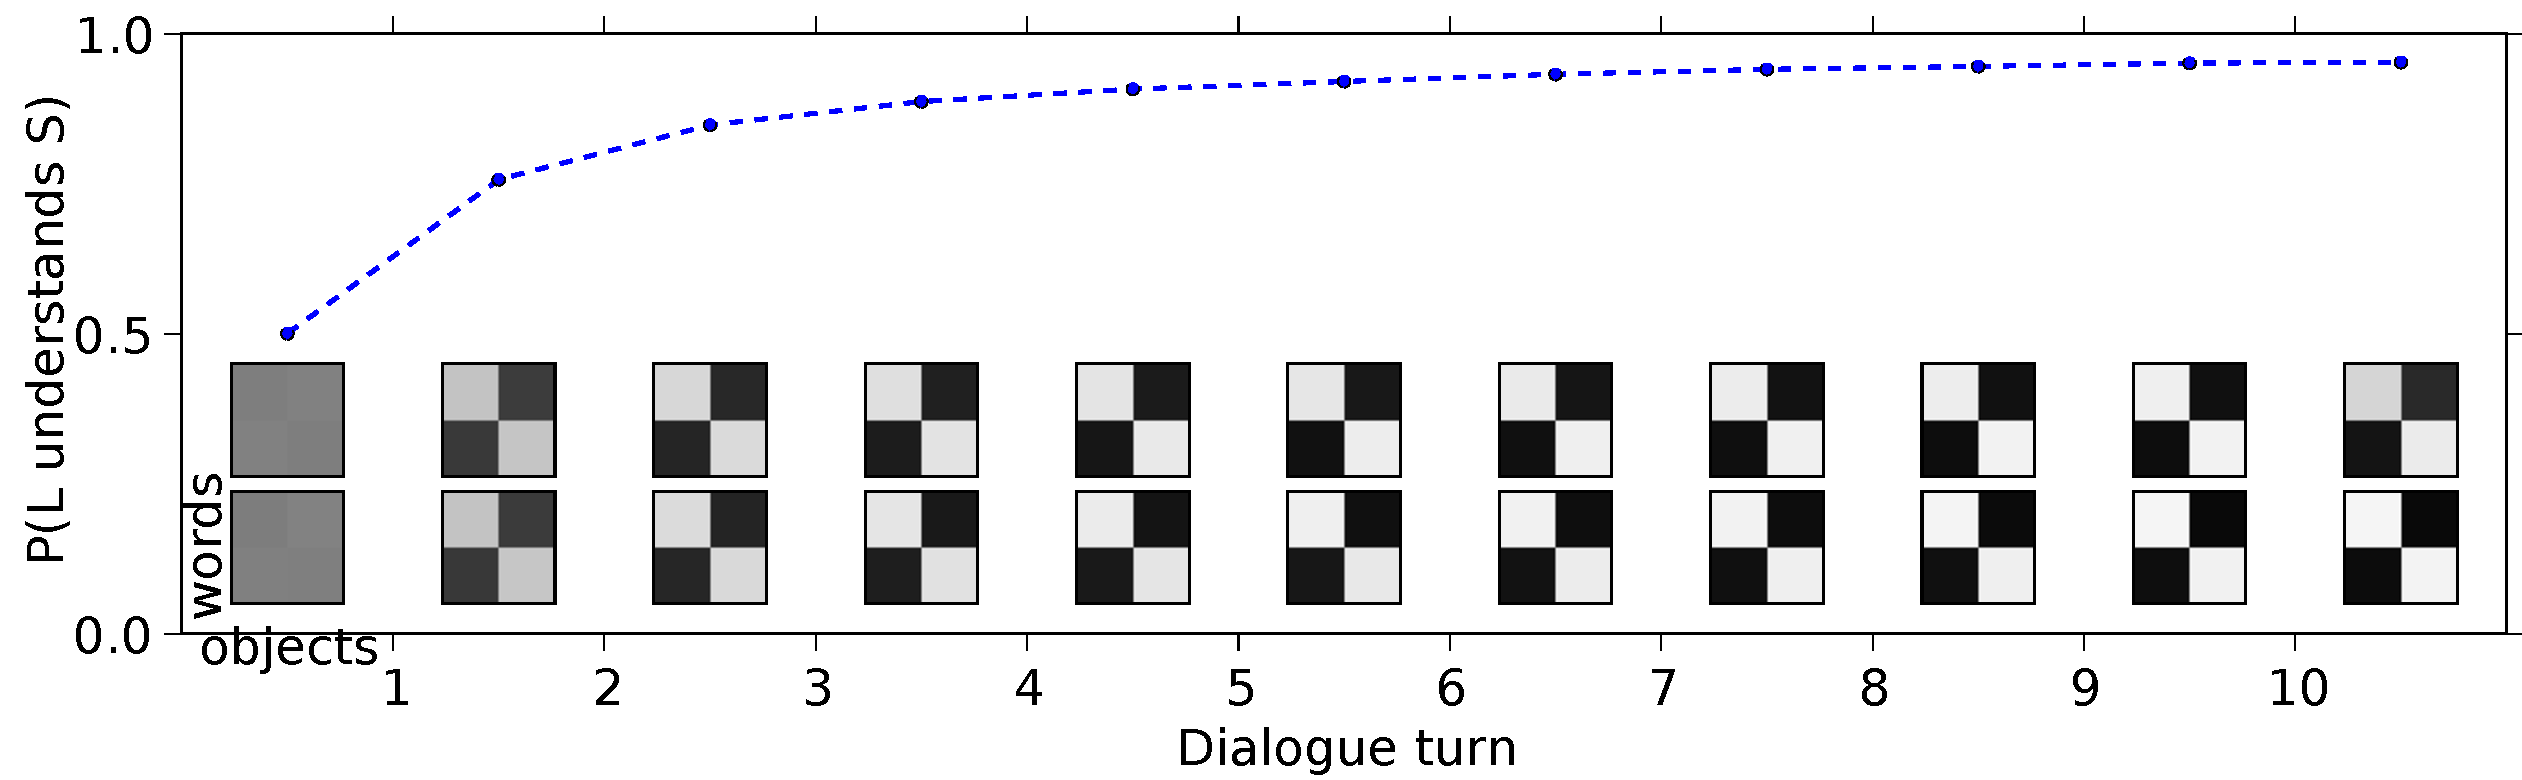
\includegraphics[width=0.48\textwidth]{figures/emergence2x2-1.pdf}
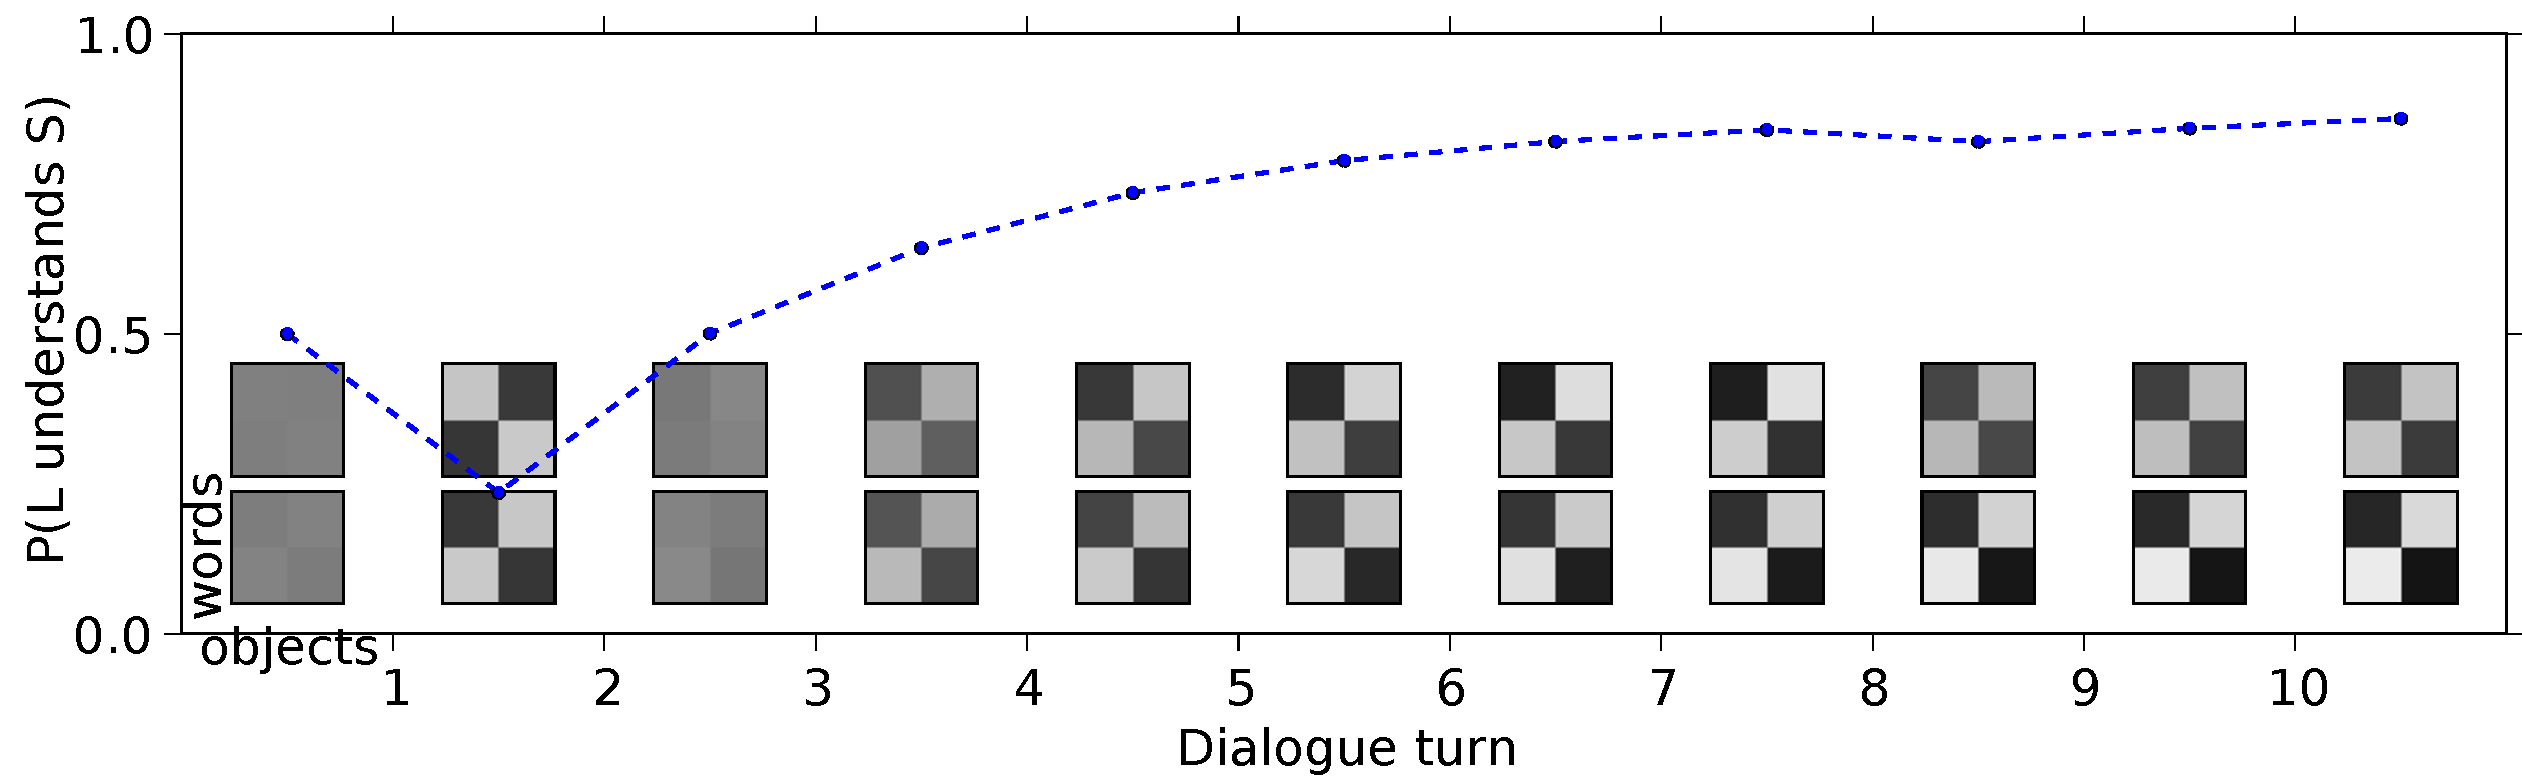
\includegraphics[width=0.48\textwidth]{figures/emergence2x2-3.pdf} \\
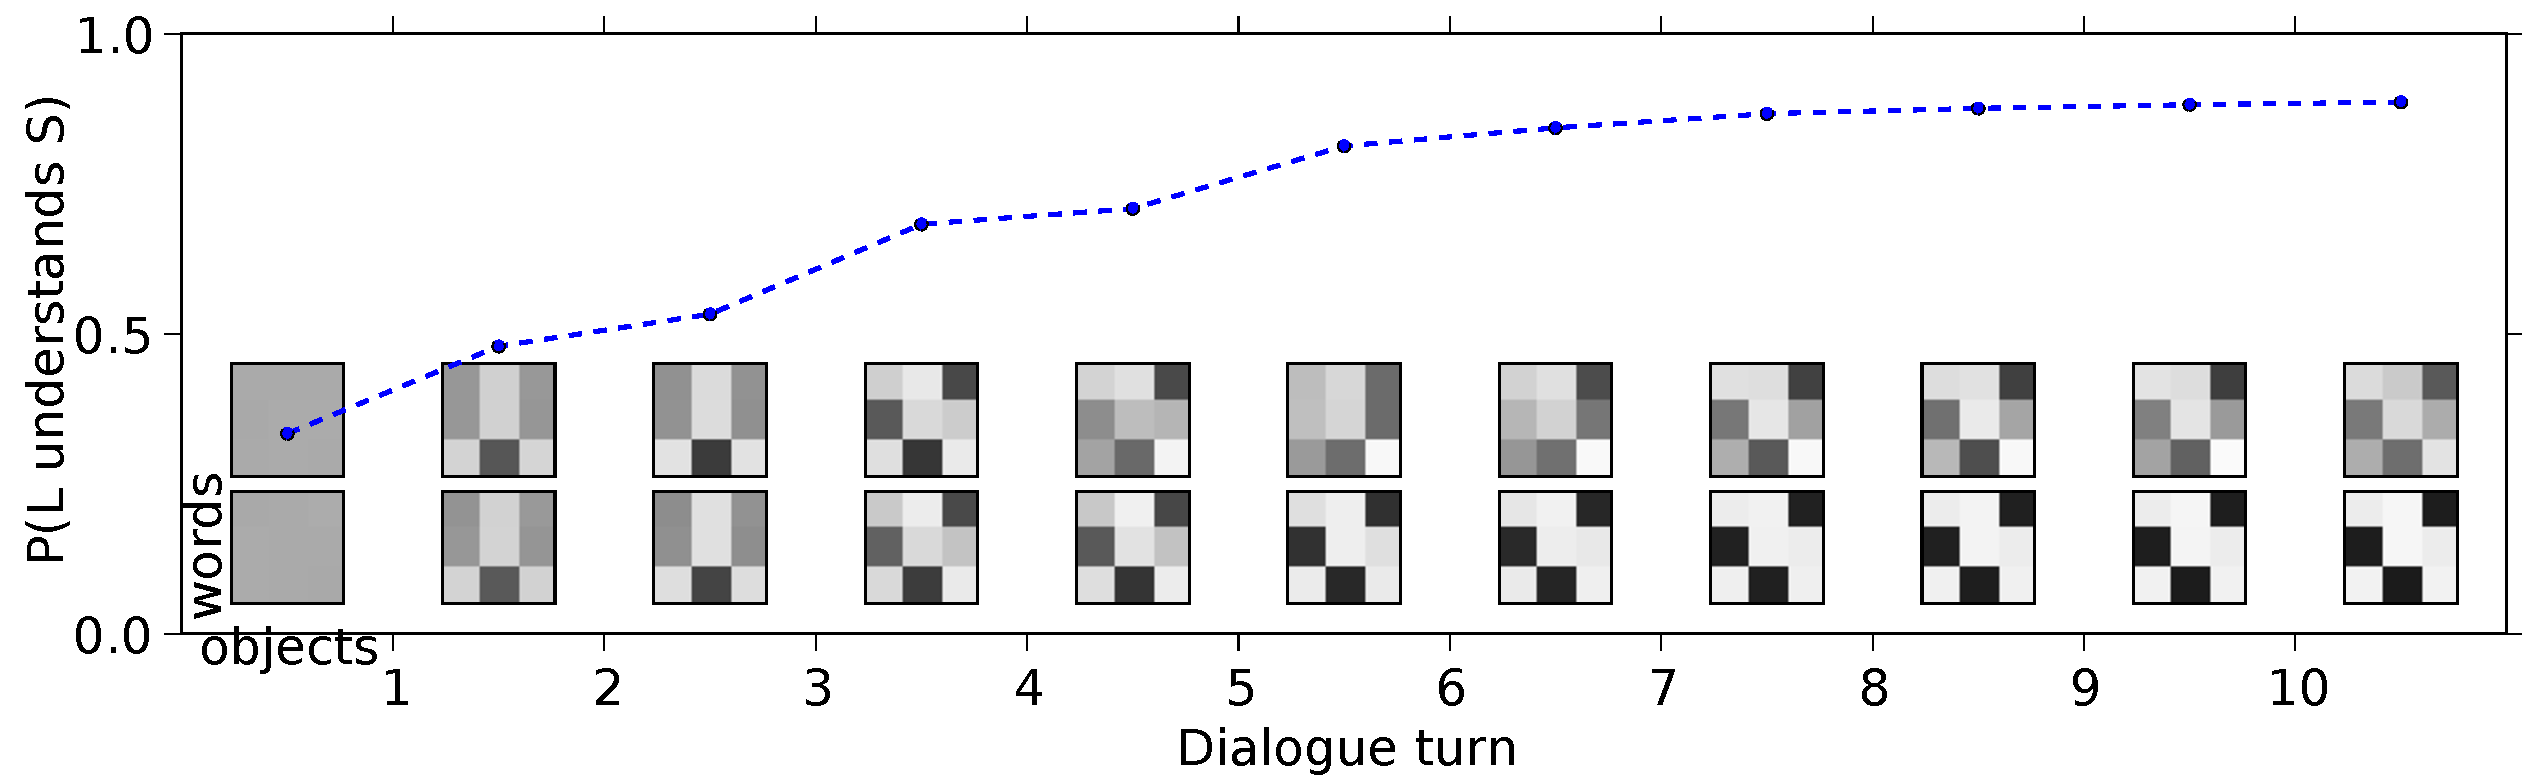
\includegraphics[width=0.48\textwidth]{figures/emergence3x3-0.pdf}
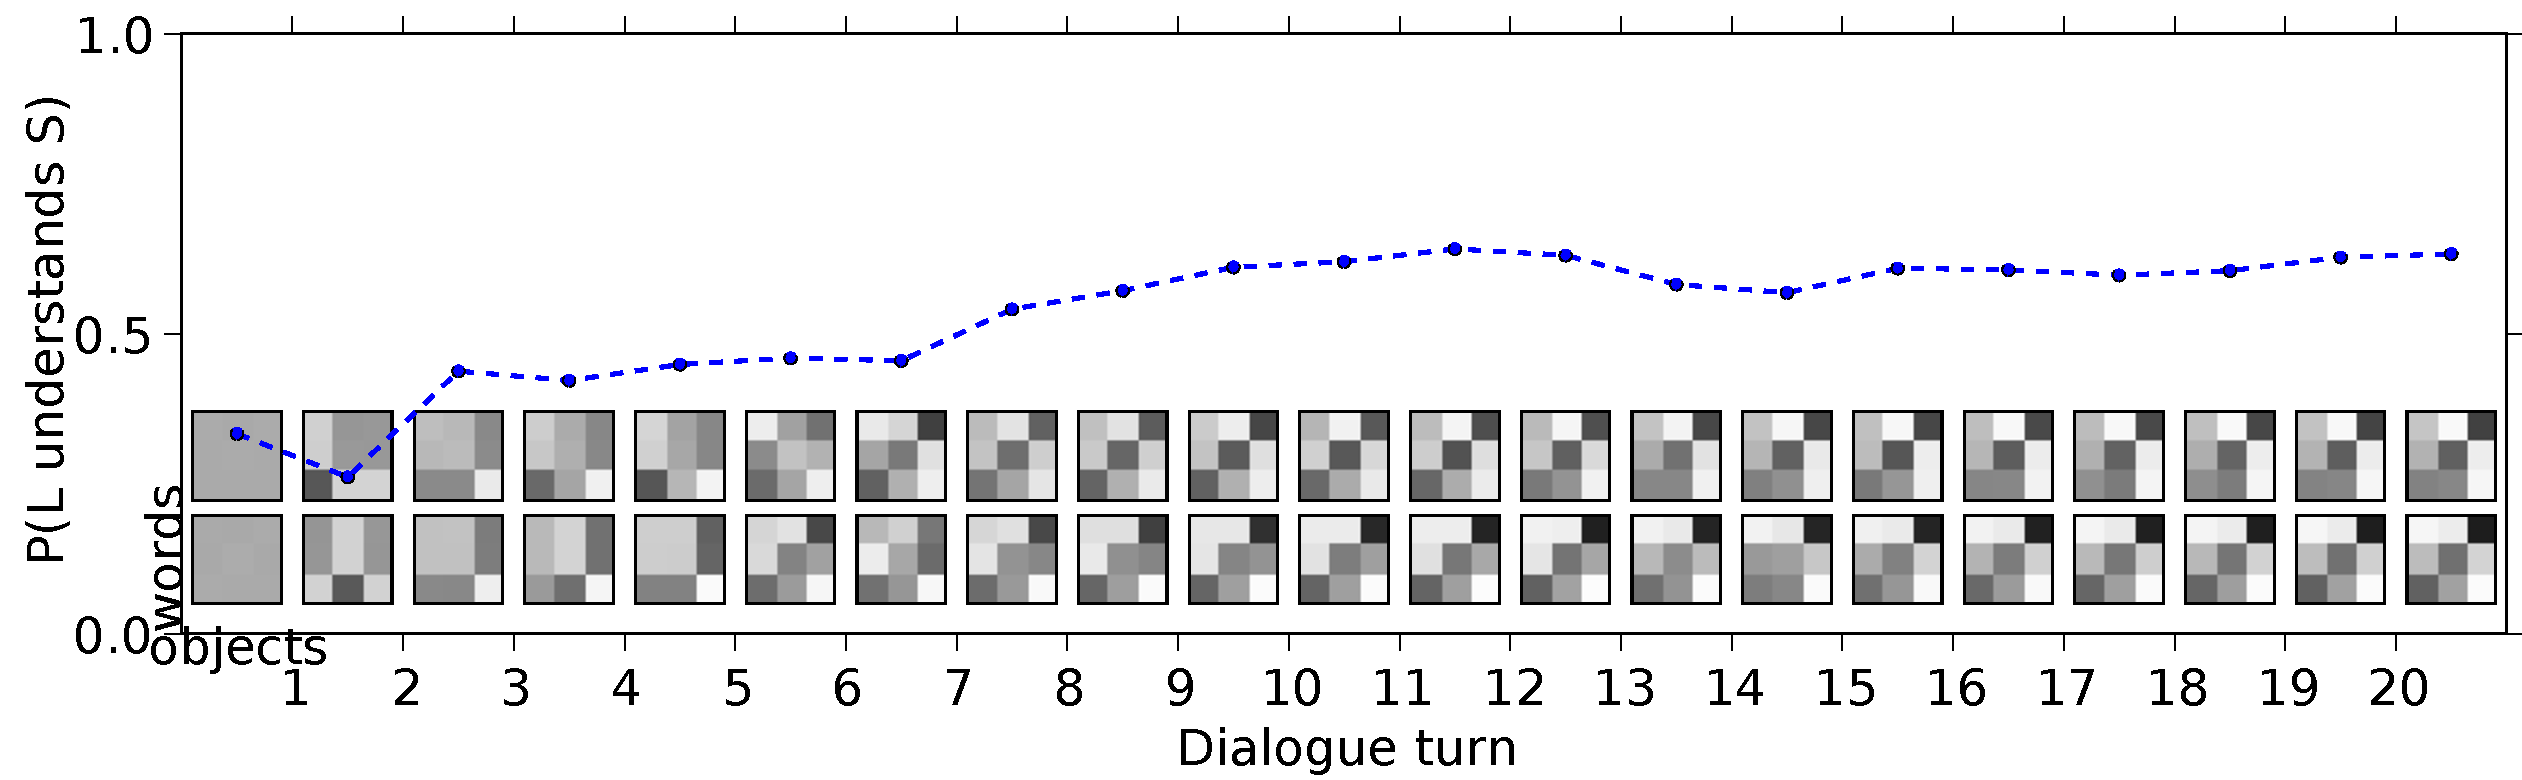
\includegraphics[width=0.48\textwidth]{figures/emergence3x3-1.pdf} \\
\caption{\label{fig:emergence} Simulations....}
\end{figure}

\subsection{Lexicalization of Horn implicatures}

\begin{figure}[t]
\centering
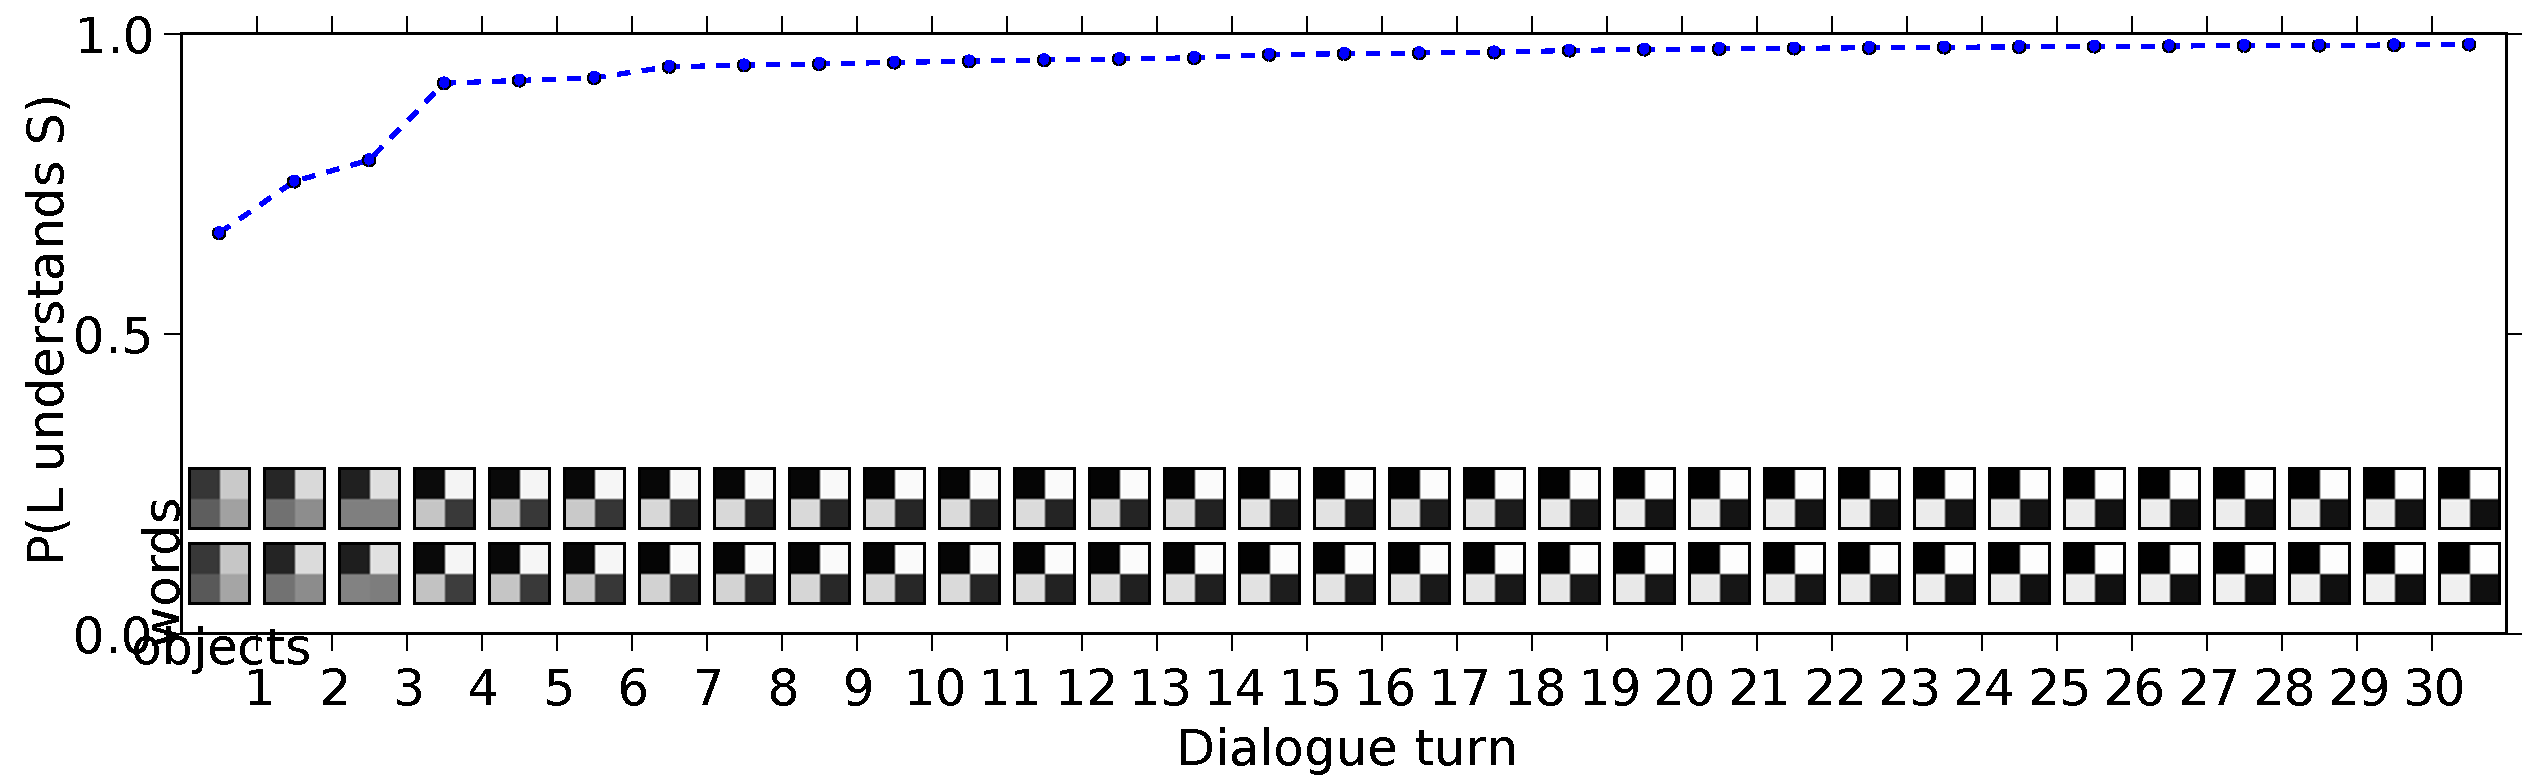
\includegraphics[width=0.48\textwidth]{figures/horn-emergence-0.pdf}
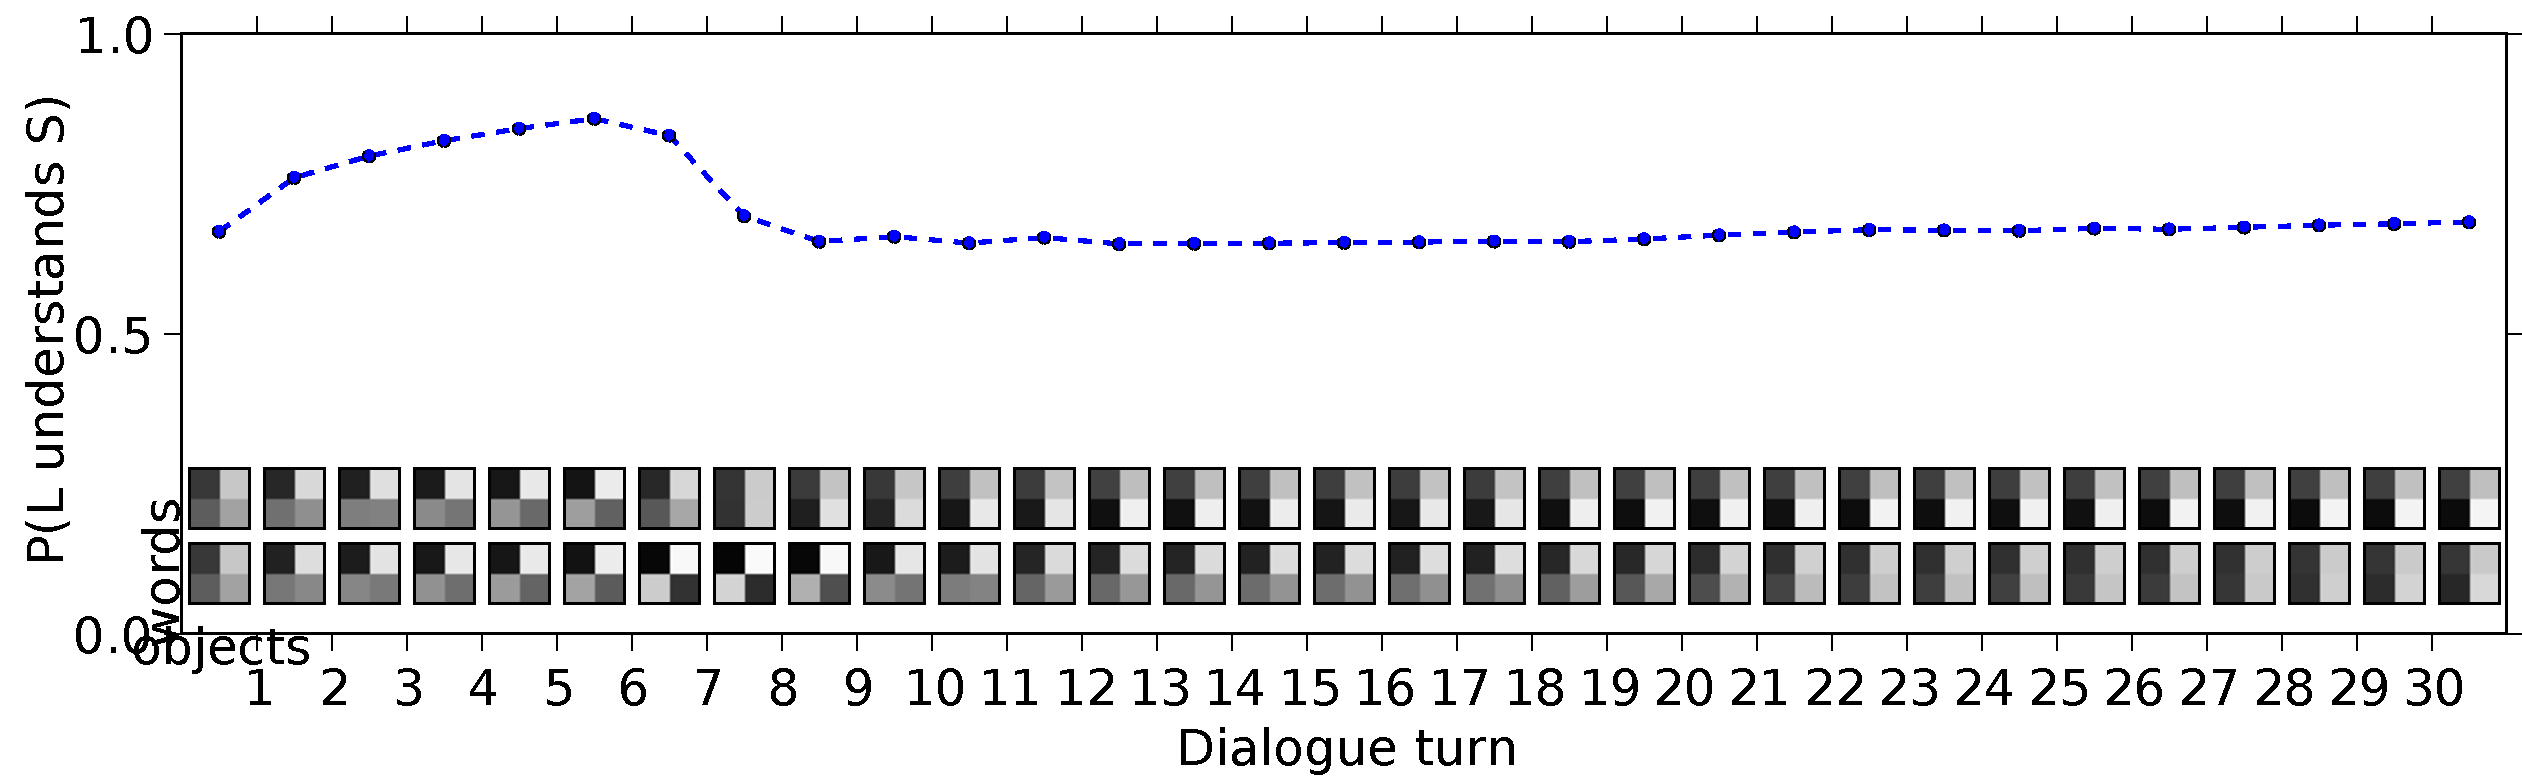
\includegraphics[width=0.48\textwidth]{figures/horn-emergence-1.pdf}
\caption{\label{fig:horn} Simulations.}
\end{figure}

% To show that they're lexicalized, at end of each of 4 dialogues, we
% look at how speaker and listener talk about/interpret the objects/words:
%
% Dialogue 0, after disabling implicature:
%   How speaker refers to "common" and "rare" objects:
% array([[  9.99994601e-01,   1.67862018e-02],
%        [  5.39888463e-06,   9.83213798e-01]])
%   Listener's interpretation of "cheap" and "expensive" words:
% array([[ 0.84765063,  0.15234937],
%        [ 0.02451694,  0.97548306]])

% Dialogue 1, after disabling implicature:
%   How speaker refers to "common" and "rare" objects:
% array([[  9.99997339e-01,   1.04639034e-02],
%        [  2.66058112e-06,   9.89536097e-01]])
%   Listener's interpretation of "cheap" and "expensive" words:
% array([[ 0.86951534,  0.13048466],
%        [ 0.01986478,  0.98013522]])

% Dialogue 2, after disabling implicature:
%   How speaker refers to "common" and "rare" objects:
% array([[  9.99984637e-01,   2.19135388e-02],
%        [  1.53629560e-05,   9.78086461e-01]])
%   Listener's interpretation of "cheap" and "expensive" words:
% array([[ 0.83486332,  0.16513668],
%        [ 0.03421814,  0.96578186]])

% Dialogue 3, after disabling implicature:
%   How speaker refers to "common" and "rare" objects:
% array([[  9.99996148e-01,   1.92821280e-02],
%        [  3.85172462e-06,   9.80717872e-01]])
%   Listener's interpretation of "cheap" and "expensive" words:
% array([[ 0.83985034,  0.16014966],
%        [ 0.02170542,  0.97829458]])


\subsection{Lexicalization and preservation of scalar implicature}


\begin{figure}
\centering
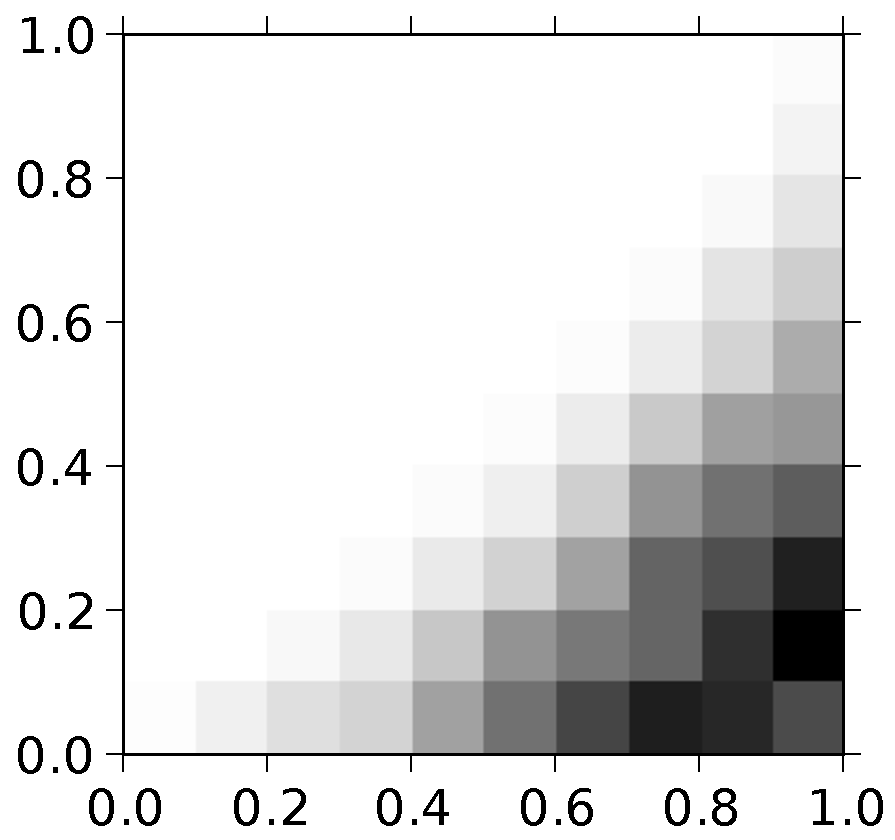
\includegraphics[width=2in]{figures/some-all-only-pragmatic.pdf}
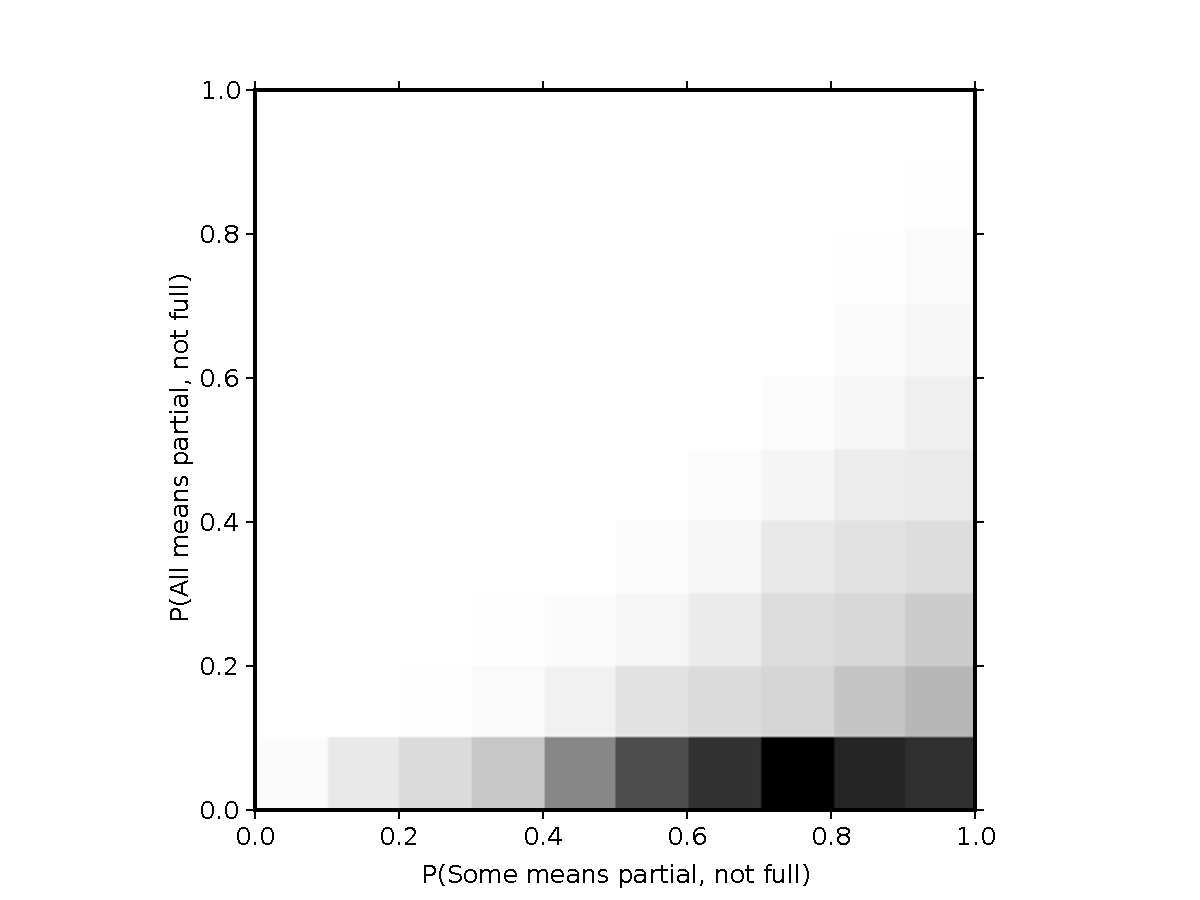
\includegraphics[width=2in]{figures/some-all-pragmatic+unambiguous.pdf}
\caption{\label{fig:scalar} Simulations..}
\end{figure}

\section{Conclusion}

%\subsubsection*{Acknowledgments}


% Thanks to ONR Grant #blahblah

\newpage

\bibliographystyle{plain}
\bibliography{pragmatics}

\end{document}
